\section{Internship accomplishments}
\label{sec:accomplish}

\subsection{Building of UI components}
\label{ssec:ui_components}

Explain the reasons behind the building of this library of static UI components

\textbf{Describe one only?}

\begin{itemize}
    \item Alert
    \item Location with GoogleMaps plugin
    \item Date/time pickers
\end{itemize}

\subsection{Implementation of new pages}
\label{ssec:new_pages}

It has been explained in {\sc subsection}~\ref{ssec:concept} that Konnektid's main goal for the year is to test and validate their business model, which relies on
professional teachers. This requires the implementation of several new pages and functionalities, and some have been built during the internship. Among them, only
two will be described here: first the course page, then the teachers landing page.

\subsubsection{The course page}
\label{sssec:coursePage}

The course page refers to the page used for teachers to create, edit and publish a course. It had to be built from scratch, for both desktop and mobile, based on designs
made by Konnektid's former designer. It is now released and used by professional teachers, and an example is visible on {\sc figure}~\ref{fig:coursePage}.

\begin{figure}[H]
    \centering
    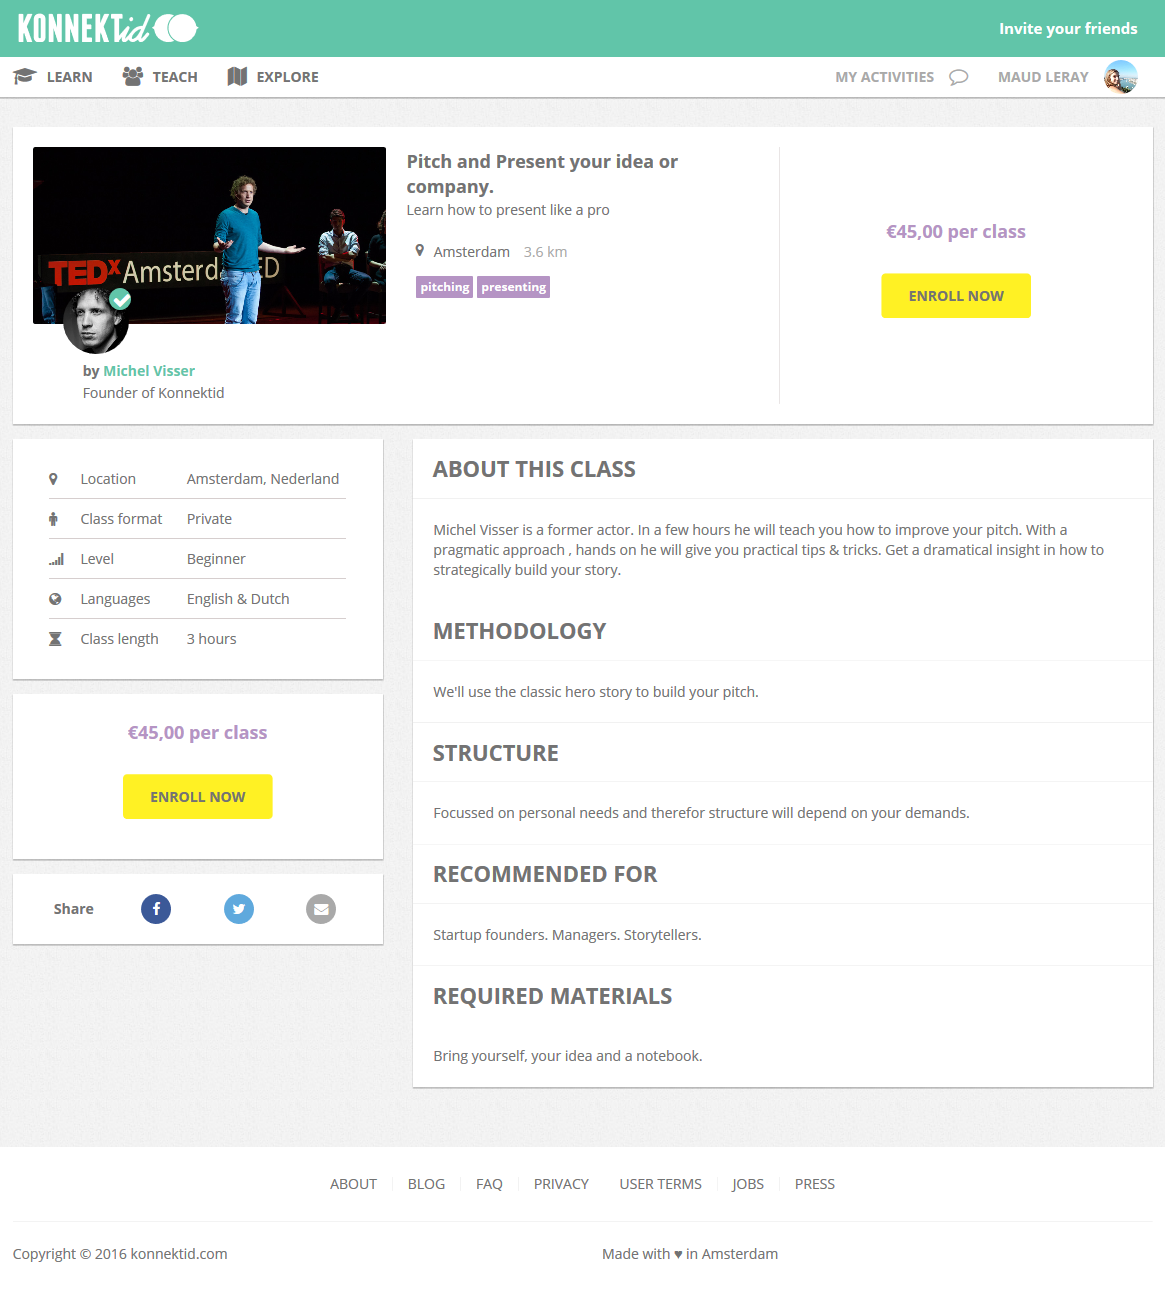
\includegraphics[scale=0.8]{figure/coursePage.png}
    \caption{An example of course published on the website (desktop version).}
    \label{fig:coursePage}
\end{figure}

We can see that the page features two main elements:

\textbf{The top section} which contains all the main information about the course (picture, title, price\ldots) and the teacher (avatar, name, short introduction).
The teacher name is a direct link to his or her profile. On the right, this section also provides a button \guillemotleft{} Enroll now \guillemotright{} for the students
to book the course.

\textbf{The bottom section} which is divided in two parts. The right part takes most space on the page and gives an in-depth description of the course
(methodology, requirements\ldots). The left part, which is thinner, shows practical information about the course (format, length\ldots) and another
\guillemotleft{} Enroll now \guillemotright{} button with a reminder of the price. Below this are all the sharing functionalities: Facebook, Twitter,
email, and even WhatsApp on mobile.

This was the very first whole JavaScript page I implemented. It made me realize the value of the components library mentioned in {\sc subsection}~\ref{ssec:ui_components}.
Indeed, it is really convenient to have all these built-in UI components to reuse, and it makes building interfaces much faster. The biggest challenge here was to divide
the page in smaller sub-components, each of them in their own folder with local CSS styles. For instance, the biggest bottom part is a component called
\guillemotleft{} CourseDescriptionCard \guillemotright{}. Since it contains several sections that are very similar in presentation and only differ by their title and content,
it made sense to create a reusable \guillemotleft{} CourseDescriptionItem \guillemotright{} to render them with title and content passed down as props. This is a recommanded
practice, as it respects the single responsibility principle previously mentioned in {\sc subsection}~\ref{ssec:frameworks} and avoids duplicated code.
These are two of the many techniques for writing maintainable code~\cite{maintainable}, i.e. code that is easy to read, to modify and to extend.

After the static course page has been built and reviewed, my tutor asked me to add inline editing for the teachers to edit their courses.
This means that all elements can be edited in-place, in the context where they will be published, which facilitates picturing the final result.
In order to implement this, I used a rich text editor framework for ReactJS called \textit{DraftJS}.

DraftJS enables the creation of rich content, such as bold or italic text and lists of items. These features are available for the teachers when editing the
CourseDescriptionCard. But they can also be blocked, for instance when editing the title of the course which needs to be a simple line.

\begin{figure}[H]
    \centering
    
\includegraphics[scale=0.8]{figure/courseEditIntro.png}
    \caption{The top section of the course page when being edited.}
    \label{fig:courseEditIntro}
\end{figure}

\subsubsection{The teachers landing page}
\label{sssec:teachersPage}

\begin{itemize}
    \item Teachers landing page => interesting because did everything from wireframe/design to implementation
\end{itemize}

\subsection{Creation of flows}
\label{ssec:flows}

\textbf{Not sure if necessary, as wireframes are already mentioned in the previous subsection?}

Matchmaking flow

\subsection{New navigation}
\label{ssec:new_nav}

\begin{itemize}
    \item Responsible of the project
    \item Added feature flag, new navigation in old pages for both mobile and desktop, only in desktop for new pages
\end{itemize}

\subsection{Analytics}
\label{ssec:analytics}

\begin{itemize}
    \item Updated analytics in old pages (for instances for inviting friends)
    \item Added analytics to new pages (explain new analytics and maybe necessary refactoring for enroll modal)
\end{itemize}
